% JUMP TO LINE 60, 73
\documentclass[preview, margin=0.6in]{standalone}
\usepackage[letterpaper,portrait,top=0.4in, left=0.6in, right=0.6in, bottom=1in]{geometry}

\usepackage{amsmath, amsfonts, amsthm, amssymb}
\usepackage{graphicx, float}
\usepackage{mathtools}
\usepackage{titlesec}
\usepackage{interval}
\usepackage{hyperref}
\usepackage{siunitx}
\usepackage{titling}
\usepackage{vwcol}
\usepackage{setspace}
\usepackage{empheq}
\usepackage{cancel}
\usepackage{esdiff}
\usepackage{multicol}
\usepackage{mdframed}
\usepackage{esdiff}
\usepackage{tikzsymbols}
\usepackage{multicol}
\usepackage{tikz}
\usepackage{varwidth}
\usepackage{pgfplots}
\pgfplotsset{compat=1.18}
\intervalconfig {
	soft open fences
}

\newcommand{\alignedintertext}[1]{%
  \noalign{%
    \vskip\belowdisplayshortskip
    \vtop{\hsize=\linewidth#1\par
    \expandafter}%
    \expandafter\prevdepth\the\prevdepth
  }%
}

\newtheorem{lemma}{Lemma}

\renewcommand{\qedsymbol}{\Smiley[1.3]}
\newcommand*{\problem}[1]{\section*{Problem #1}}
\newcommand*{\aps}{\section*{AP Corner}}
\newcommand*{\deriv}[1][x]{\ensuremath{\dfrac{\mathrm{d}}{\mathrm{d}#1}}}
\newcommand*{\floor}[1]{\ensuremath{\lfloor #1\rfloor}}
\newcommand*{\lheqzero}{\ensuremath{\underset{\text{L'H}}{\overset{\left[\frac00\right]}{=}}}}
\newcommand*{\lheqinfty}{\ensuremath{\underset{\text{L'H}}{\overset{\left[\frac{\infty}{\infty}\right]}{=}}}}

\DeclareMathOperator{\DNE}{DNE}
\DeclareMathOperator{\sgn}{sgn}

\DeclareMathOperator{\arccsc}{arccsc}
\DeclareMathOperator{\arcsec}{arcsec}
\DeclareMathOperator{\arccot}{arccot}

\setlength{\parindent}{0pt}

%opening
\title{\vspace*{-30pt}Problem Set \#28}
\author{Jayden Li}
\date{\today}

% \allowdisplaybreaks
\postdisplaypenalty=100000

\begin{document}
\setstretch{1.25}
\fontsize{12pt}{12pt}\selectfont
\setlength{\abovedisplayskip}{0pt}
\maketitle
\problem{6}
$y=r$ is perpendicular to the $y$-axis, so we will use $\mathrm dx$.

\begin{center}
	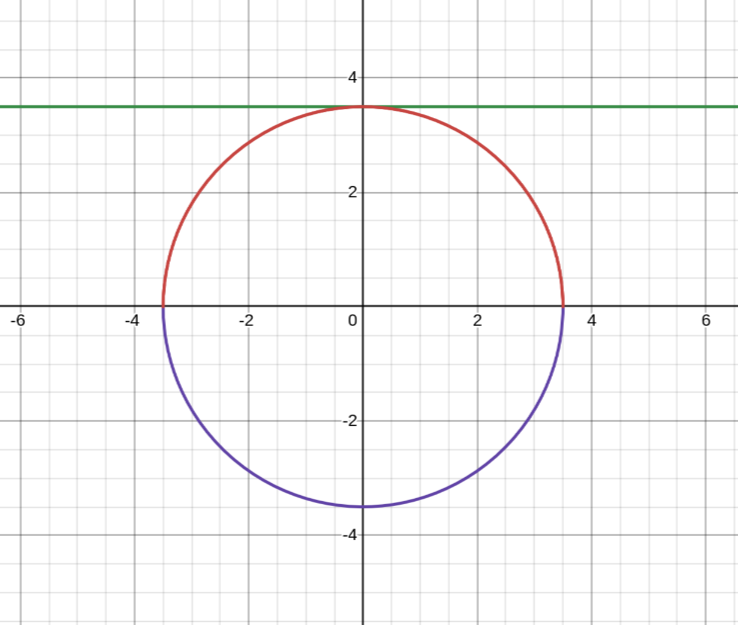
\includegraphics[width=0.5\linewidth]{p6.png}
\end{center}

$\begin{aligned}[t]
	&x^2+y^2=r^2
	\implies y=\pm \sqrt{r^2-x^2}
	\implies \diff yx=\pm \frac{-2x}{2 \sqrt{r^2-x^2}}
	=\mp \frac{x}{\sqrt{r^2-x^2}}
\end{aligned}$

$\begin{aligned}[t]
	S_{\text{red}}&=\int_{-r}^{r} 2\pi\cdot\text{radius}\cdot \sqrt{1+\left(\diff yx\right)^2}\,\mathrm{d}x \\
	\alignedintertext{Radius is distance between $y=r$ and the circle, which is $r- \sqrt{r^2-x^2}$.}
	&=\int_{-r}^{r}2\pi \left(r-\sqrt{r^2-x^2}\right)\sqrt{1+\left(\mp \frac{x}{\sqrt{r^2-x^2}}\right)^2}\,\mathrm{d}x
	=\boxed{2\pi\int_{-r}^{r}\left(r-\sqrt{r^2-x^2}\right)\sqrt{1+\frac{x^2}{r^2-x^2}}\,\mathrm{d}x} \\
	&=2\pi \int_{-r}^{r}\left(r \sqrt{1+\frac{x^2}{r^2-x^2}}-\sqrt{r^2-x^2+\frac{x^2}{\cancel{r^2-x^2}}\cdot \left(\cancel{r^2-x^2}\right)}\right)\mathrm{d}x \\
	&=2\pi \int_{-r}^{r}\left(r \sqrt{\frac{r^2-x^2}{r^2-x^2}+\frac{x^2}{r^2-x^2}}-\sqrt{r^2-x^2+x^2}\right)\mathrm{d}x
	=2\pi \int_{-r}^{r}\left(r \sqrt{\frac{r^2}{r^2-x^2}}-r\right)\mathrm{d}x \\
	&=2\pi r \int_{-r}^{r}\left(\frac{r}{\sqrt{r^2-x^2}}-1\right)\mathrm{d}x
	=2\pi r \int_{-r}^{r}\left(\frac{\cancel{r}}{\cancel{r}\sqrt{1-\frac{x^2}{r^2}}}-1\right)\mathrm{d}x \\
	&=\left[\begin{aligned}
			u&=x/r \\
			\mathrm{d}u&=\mathrm{d}x/r
	\end{aligned}\right]
	2\pi r^2 \int_{-1}^{1}\left(\frac{1}{\sqrt{1-u^2}}-1\right)\mathrm{d}u
	=2\pi r^2 \Big[\arcsin u-u\Big]_{-1}^{1} \\
	&=2\pi r^2 \left(\frac{\pi}{2}-1-\left(-\frac{\pi}{2}-(-1)\right)\right)
	=2\pi r^2 \left(\frac{\pi}{2}-1+\frac{\pi}{2}-1\right)
	=2\pi r^2 (\pi-2) \\ 
	\alignedintertext{Notice that the ``radius'' of revolution for the purple curve (whose equation is $y=- \sqrt{r^2-x^2}$) is $r+\left|y\right|=r+\left|-\sqrt{r^2-x^2}\right|=r+\sqrt{r^2-x^2}$.}
	S_{\text{purple}}&=\int_{-r}^{r}2\pi \left(r+\sqrt{r^2-x^2}\right)\sqrt{1+\left(\mp \frac{x}{\sqrt{r^2-x^2}}\right)^2}\,\mathrm{d}x
	=2\pi \int_{-r}^{r}\left(r+\sqrt{r^2-x^2}\right)\sqrt{1+\frac{x^2}{r^2-x^2}}\,\mathrm{d}x \\
	\alignedintertext{Notice this differs from the above boxed expression by only a plus sign.}
	&=2\pi \int_{-r}^{r}\left(\frac{r}{\sqrt{r^2-x^2}}+1\right)\,\mathrm{d}x
	=\ldots=2\pi r^2 \Big[\arcsin u+u\Big]_{-1}^{1}
	= 2\pi r^2 \left(\frac{\pi}{2}+1-\left(-\frac{\pi}{2}-1\right)\right) \\
	&=2\pi r^2 \left(\frac{\pi}{2}+1+\frac{\pi}{2}+1\right)
	=2\pi r^2 (\pi+2) \\
	\alignedintertext{Total surface area is the sum of the surface areas of the two individual solids.}
	S&=S_{\text{red}}+S_{\text{purple}}
	=2\pi r^2(\pi-2)+2\pi r^2(\pi+2)
	=2\pi^2r^2-\cancel{4\pi r^2}+2\pi^2r^2+\cancel{4\pi r^2}
	=\boxed{4\pi^2r^2}
\end{aligned}$

\end{document}
